\documentclass{article}
\usepackage[utf8]{inputenc}
\usepackage{graphicx}
\usepackage{amsmath}
\usepackage{titling}
\usepackage{pdflscape}
\usepackage[export]{adjustbox}
\usepackage{float}

\setlength{\droptitle}{-10em}
\pagestyle{empty}

\title{Lab. 2 - La rete dei trasporti pubblici}
\author{Ballarin Simone, Gobbo Alessio, Rossi Daniel}
\date{April 2019}

\begin{document}
\maketitle

\section*{Domanda 1}
La rete di traporti è stata modellata come un multi grafo orientato con archi pesati, abbiamo considerato il grafo così organizzato:
\begin{itemize}
	\item \textbf{Vertici}: stazioni della rete;
	\item \textbf{Archi}: trasporti disponibili tra una stazione ed un'altra.
\end{itemize}

Scendendo maggiormente nel dettaglio ogni nodo (stazione) ha per lista delle adiacenze un dizionario, questo ha per chiave il codice della stazione di arrivo e per valore una lista ordinata, per orario di partenza, delle corse con partenza dalla stazione corrente a quella chiave.
Si è quindi deciso di utilizzare come peso per ciascun arco l'orario di arrivo di un trasporto alla stazione destinazione.

\section*{Domanda 2}
Abbiamo implementato sia l'algoritmo Dijkstra che l'algoritmo A* utilizzando per entrambi una coda di priorità.
Rispetto l'algoritmo generico visto a lezione si è deciso di inglobare la funzione di inizializzazione e quella di rilassamento all'interno della struttura dati di appoggio.\\
La struttura dati considera considera come priorità l'orario associato ai nodi presenti nella coda, l'ora considerata è quella minima rispettivamente:
\begin{itemize}
	\item Dijkstra: ora localmente minore di arrivo alla stazione stessa;
	\item A*: ora stimata di arrivo alla stazione di destinazione dalla stazione stessa.
\end{itemize}
I due algoritmi forniscono le stesse soluzioni alle stesse istanze di problemi. L'euristica è calcolata come il tempo necessario a percorrere alla velocità di 300 km/h la distanza in linea d'aria tra due nodi. La funzione di valutazione di conseguenza consiste nella somma all'ora di arrivo a una determinata stazione di questa euristica, fornendo così un'ora stimata di arrivo. Con punti poco lontani A* presenta un notevole vantaggio in termini di tempo di esecuzione, mentre scegliendo stazioni molto lontane  A* presenta tempi peggiori. Abbiamo quindi deciso di calcolare il tempo impiegato da A* non considerando il tempo di calcolo dell'euristica. Il tempo così ottenuto è estremamente vicino al tempo di Dijkstra (leggermente inferiore), questo ci ha quindi portato a concludere che con punti lontani l'euristica risulti ingannevole e quindi porta a intraprendere molti percorsi errati arrivando alla stessa complessità di Dijkstra con però l'aggiunta di un notevole overhead dovuto al calcolo dell'euristica.
\newpage
\section*{Domanda 3}
\begin{figure}[H]
	\begin{minipage}{0.55\linewidth}
		\centering
		\hspace*{-3cm}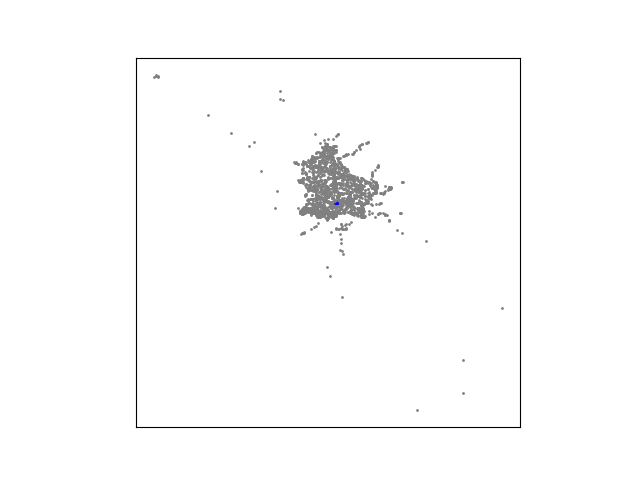
\includegraphics[width=1.0\linewidth, valign=t]{figures/200415016_200405005}
	\end{minipage}
	\hspace*{-2cm}\begin{minipage}{0.7\linewidth}
		\textbf{Viaggio da 200415016 a 200405005}:\\
		Orario di partenza: 09:30\\
		Orario di arrivo: 09:52\\
		\mbox{09:30 corsa 00360 RGTR125/1 da 200415016 a 200415009}\\
		09:50 corsa 06602 RGTR10 da 200415009 a 200405005
			\end{minipage}
\end{figure}
\begin{figure}[H]
	\begin{minipage}{0.55\linewidth}
		\centering
		\hspace*{-3cm}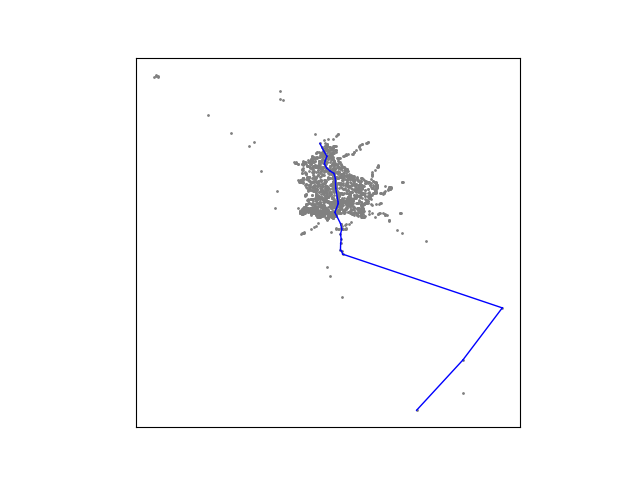
\includegraphics[width=1.0\linewidth, valign=t]{figures/300000032_400000122}
	\end{minipage}
	\hspace*{-2cm}\begin{minipage}{0.7\linewidth}
		\textbf{Viaggio da 300000032 a 400000122}:\\
		Orario di partenza: 05:30\\
		Orario di arrivo: 13:50\\
		06:26 corsa 07608 C881 da 300000032 a 110606001\\
		07:26 corsa 03781 C821 da 110606001 a 200417051\\
		07:46 corsa 00055 C82TER da 200417051 a 220102005\\
		12:07 corsa 09879 C821 da 220102005 a 400000122
		
			\end{minipage}
\end{figure}
\begin{figure}[H]
	\begin{minipage}{0.55\linewidth}
		\centering
		\hspace*{-3cm}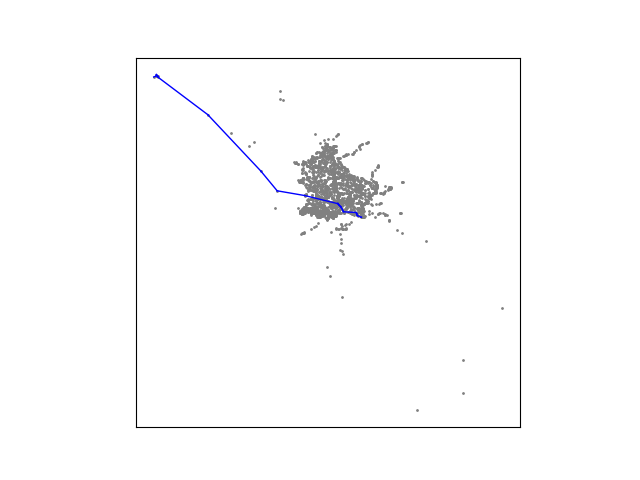
\includegraphics[width=1.0\linewidth, valign=t]{figures/210602003_300000030}
	\end{minipage}
	\hspace*{-2cm}\begin{minipage}{0.7\linewidth}
		\textbf{Viaggio da 210602003 a 300000030}:\\
		Orario di partenza: 06:30\\
		Orario di arrivo: 10:53\\
		\mbox{06:41 corsa 00030 CFLBUS185 da 210602003 a 210602005}\\
		\mbox{06:55 corsa 00037 CFLBUS175 da 210602005 a 220502003}\\
		\mbox{07:07 corsa 01306 CFLBUS176 da 220502003 a 201103001}\\
		07:20 corsa 00024 RGTR176 da 201103001 a 200405036\\
		07:24 corsa 01173 RGTR172 da 200405036 a 200405026\\
		07:27 corsa 04301 AVL31 da 200405026 a 200405035\\
		07:40 corsa 07630 C821 da 200405035 a 300000030
			\end{minipage}
\end{figure}
\begin{figure}[H]
	\begin{minipage}{0.55\linewidth}
		\centering
		\hspace*{-3cm}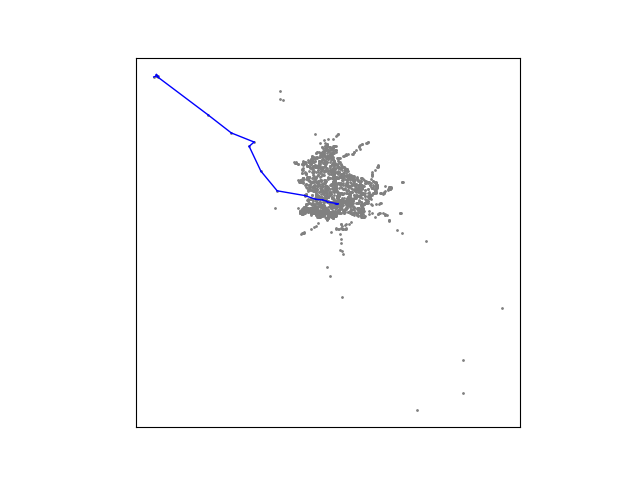
\includegraphics[width=1.0\linewidth, valign=t]{figures/200415009_300000030}
	\end{minipage}
	\hspace*{-2cm}\begin{minipage}{0.7\linewidth}
		\textbf{Viaggio da 200415009 a 300000030}:\\
		Orario di partenza: 18:00\\
		Orario di arrivo: 22:28\\
		\mbox{18:08 corsa 00350 RGTR125/1 da 200415009 a 200415017}\\
		18:13 corsa 08140 RGTR27 da 200415017 a 200405035\\
		18:22 corsa 05838 C821 da 200405035 a 200101007\\
		19:31 corsa 02142 C821 da 200101007 a 300000030
		
		
			\end{minipage}
\end{figure}
\begin{figure}[H]
	\begin{minipage}{0.55\linewidth}
		\centering
		\hspace*{-3cm}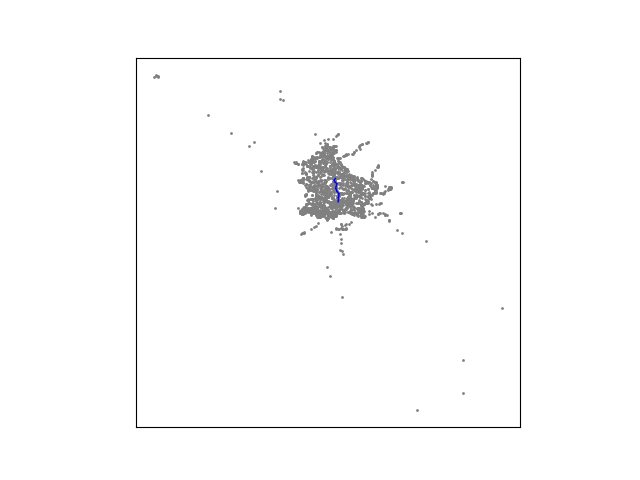
\includegraphics[width=1.0\linewidth, valign=t]{figures/200417051_140701016}
	\end{minipage}
	\hspace*{-2cm}\begin{minipage}{0.7\linewidth}
		\textbf{Viaggio da 200417051 a 140701016}:\\
		Orario di partenza: 23:55\\
		Orario di arrivo: 00:44\\
		00:09 corsa 03623 C821 da 200417051 a 140701016
		
	\end{minipage}
\end{figure}
\begin{figure}[H]
	\begin{minipage}{0.55\linewidth}
		\centering
		\hspace*{-3cm}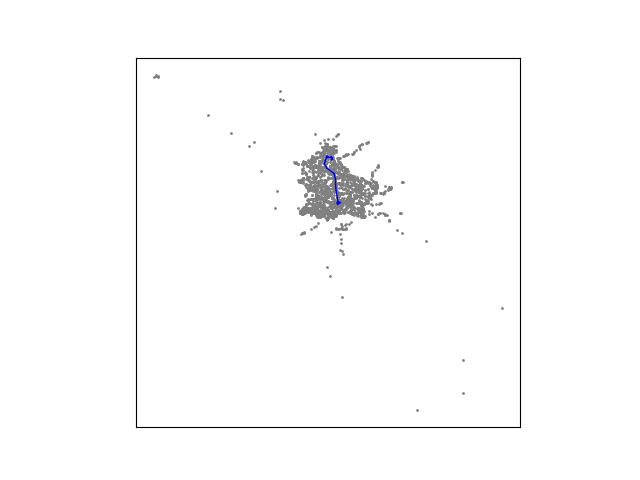
\includegraphics[width=1.0\linewidth, valign=t]{figures/200406015_110405001}
	\end{minipage}
	\hspace*{-2cm}\begin{minipage}{0.7\linewidth}
		\textbf{Viaggio da 200406015 a 110405001}:\\
		Orario di partenza: 21:30\\
		Orario di arrivo: 07:16\\
		21:45 corsa 02708 AVL20 da 200406015 a 200406013\\
		21:47 corsa 03714 AVLCN da 200406013 a 200406011\\
		\mbox{21:57 corsa 00487 RGTR125/1 da 200406011 a 200405020}\\
		22:03 corsa 03714 AVLCN da 200405020 a 200405023\\
		22:12 corsa 03725 AVLCN da 200405023 a 200405035\\
		22:16 corsa 03722 C821 da 200405035 a 200417051\\
		04:30 corsa 03468 RGTR840 da 200417051 a 110101004\\
		07:14 corsa 02156 RGTR665 da 110101004 a 110405001
		
\end{minipage}
\end{figure}
\begin{figure}[H]
	\begin{minipage}{0.55\linewidth}
		\centering
		\hspace*{-3cm}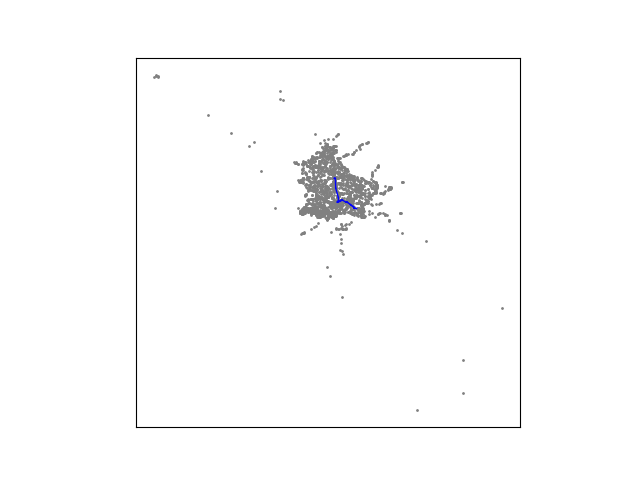
\includegraphics[width=1.0\linewidth, valign=t]{figures/140701040_210101001}
	\end{minipage}
	\hspace*{-2cm}\begin{minipage}{0.7\linewidth}
		\textbf{Viaggio da 140701040 a 210101001}:\\
		Orario di partenza: 05:30\\
		Orario di arrivo: 07:10\\
		05:34 corsa 06082 RGTR512 da 140701040 a 140701013\\
		05:45 corsa 03830 C821 da 140701013 a 160904001\\
		\mbox{06:12 corsa 03626 CFLBUSL10 da 160904001 a 200419026}\\
		06:20 corsa 03177 AVL4 da 200419026 a 200405014\\
		06:22 corsa 00040 AVL18 da 200405014 a 200417047\\
		06:34 corsa 05313 RGTR213 da 200417047 a 200417044\\
		06:41 corsa 00693 RGTR194 da 200417044 a 200601006\\
		06:51 corsa 02907 RGTR160 da 200601006 a 210101001
		
			\end{minipage}
\end{figure}
\begin{figure}[H]
	\begin{minipage}{0.55\linewidth}
		\centering
		\hspace*{-3cm}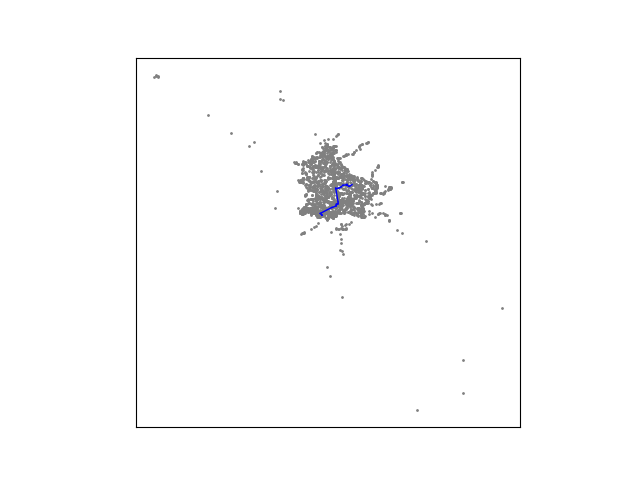
\includegraphics[width=1.0\linewidth, valign=t]{figures/170801001_220402082}
	\end{minipage}
	\hspace*{-2cm}\begin{minipage}{0.7\linewidth}
		\textbf{Viaggio da 170801001 a 220402082}:\\
		Orario di partenza: 12:30\\
		Orario di arrivo: 14:44\\
		12:45 corsa 03018 RGTR414 da 170801001 a 160501003\\
		12:59 corsa 01007 RGTR100 da 160501003 a 160601001\\
		13:07 corsa 01473 RGTR409 da 160601001 a 160601008\\
		13:26 corsa 03737 C821 da 160601008 a 200417051\\
		13:44 corsa 08000 RGTR27 da 200417051 a 200415003\\
		13:46 corsa 07810 RGTR200 da 200415003 a 200415002\\
		13:58 corsa 05168 RGTR205 da 200415002 a 220701003\\
		14:11 corsa 07234 RGTR321 da 220701003 a 220402106\\
		14:42 corsa 00056 TIC12 da 220402106 a 220402082
		
			\end{minipage}
\end{figure}

\section*{Domanda 4}
Le soluzioni fornite dagli algoritmi sono ottime, sotto l'assunzione che il tempo di spostamento all'interno delle stazioni, da un binario ad un altro per esempio, sia nullo e che quindi non venga considerato.\\
Un possibile miglioramento per rendere più ragionevoli alcune soluzioni potrebbe essere quello di minimizzare il numero di cambi, questo perché dato un percorso ottimo potrebbe esisterne uno che arriva alla stessa destinazione poco tempo dopo ma facendo un numero minore di cambi.\\
Questa modifica potrebbe essere fatta assegnando una penalità oraria (ritardo) se si effettua il cambio, si dovrebbe quindi incrementare di una certa quantità $k$ l'orario di partenza da quella stazione se non si prosegue con la stessa corsa con cui si è arrivati.\\
Un altro problema riscontrabile nell'utilizzo di soluzioni ottime fornite dagli algoritmi, su stesse istanze del problema, è la restituzione della stessa soluzione di viaggio ottima per ogni ricerca, questo potrebbe portare ad un sovraffollamento di alcune corse generando ritardi e disservizi della rete, quindi una possibile soluzione potrebbe essere quella di considerare tutte le soluzioni ottime fornite per uno stesso problema e bilanciare il carico sulle diverse soluzioni.

\section*{Domanda 5}
In allegato alla consegna sono stati inseriti i codice sorgente Python.

\end{document}
